\documentclass{article}
\usepackage{tikz}
\usepackage{amsmath}
\usepackage{mathtools}
\DeclarePairedDelimiter\ceil{\lceil}{\rceil}
\DeclarePairedDelimiter\floor{\lfloor}{\rfloor}

\usetikzlibrary{automata,arrows,er,fit,intersections,positioning,snakes,shapes,trees}

\usetikzlibrary{external}
\tikzexternalize[prefix=figures/]{main} % provide the file’s real name
\begin{document}

{
\tikzsetfigurename{figure_}

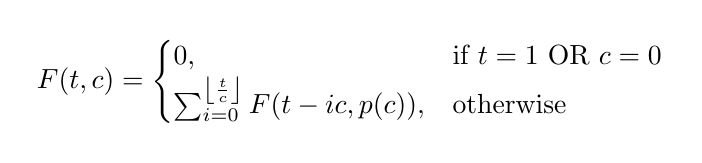
\begin{tikzpicture}
\node (x1) {
$F(t, c)=
\begin{cases}
0,                               & \text{if } t = 1 \text{ OR } c = 0\\
\sum_{i=0}^{\floor*{\frac{t}{c}}} F(t - ic, p(c)), & \text{otherwise}
\end{cases}
$};
\end{tikzpicture}

% f(x)=
% \begin{cases}
%     \frac{x^2-x}{x},& \text{if } x\geq 1\\
%     0,              & \text{otherwise}
% \end{cases}


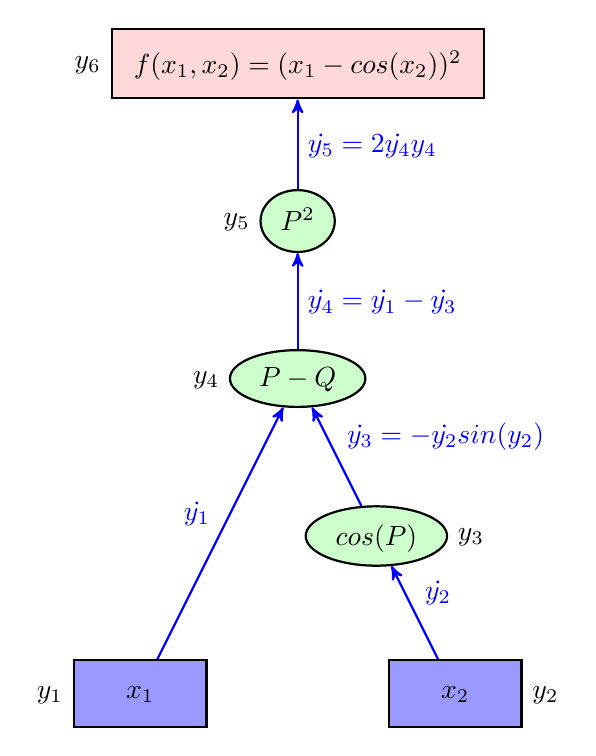
\begin{tikzpicture}
[>=stealth',auto,text depth=1pt,
every attribute/.style={fill=green!20,draw=black,thick},
every entity/.style={inner sep=0pt,fill=blue!40,draw=black,thick},
every relationship/.style={inner sep=8pt,rectangle,fill=red!15,draw=black,thick},
pre/.style={<-,shorten <=1pt,>=stealth’,semithick}
]
\node[entity] (x1) at (0,0) [label=left:$y_1$] {$x_1$};
\node[entity] (x2) at (4,0) [label=right:$y_2$] {$x_2$};
\node[attribute] (cosp) at (3,2) [label=right:$y_3$] {$cos(P)$};
\node[attribute] (pq) at (2,4) [label=left:$y_4$] {$P-Q$};
\node[attribute] (p2) at (2,6) [label=left:$y_5$] {$P^2$};
\node[relationship] (fonction) at (2,8) [label=left:$y_6$] {$f(x_1,x_2)= (x_1-cos(x_2))^2$};


\path[->,thick,blue] (x1) edge node {$\dot{y_1} $} (pq);
\path[->,thick,blue] (x2) edge node [swap] {$\dot{y_2} $} (cosp);
\path[->,thick,blue] (cosp) edge node [swap] {$\dot{y_3}=-\dot{y_2}sin(y_2)$} (pq);
\path[->,thick,blue] (pq) edge node [swap] {$\dot{y_4}=\dot{y_1}-\dot{y_3}$} (p2);
\path[->,thick,blue] (p2) edge node [swap] {$\dot{y_5}=2\dot{y_4}y_4$} (fonction);
\end{tikzpicture}

\def\xmin{-1}
\def\xmax{4}
\def\xk1{1.2894652}

\begin{tikzpicture}[samples=100,domain=\xmin:\xmax]
\draw[very thin,color=gray] (-0.2,-0.5) grid (4.2,4);
\draw[->] ({\xmin-0.1},0) -- ({\xmax+0.1},0) node[right] {$x$};
\draw[->] (0,-1) -- (0,4) node[above] {$F(x)$};
\draw[color=blue] plot (\x,{(-3*sin(\x r)+4*\x)/6}) node[right] {$F(x)$};
\draw[-] (3.5,0) node[below] {$x_k$} -- (3.5,{(-3*sin(3.5 r)+4*(3.5))/6});
\begin{scope}
%\clip (-3.5,0) rectangle (0,5);
\clip (0,0) rectangle (3.5,4);
\draw[color=red] plot (\x,{(-3*sin(3.5 r)+4*(3.5) + (-3*cos(\x-3.5 r)+4)*(\x-3.5))/6});
\end{scope}
\node [below] at (\xk1,0)  {$x_{k+1}$};



\draw[-] (\xk1,0) -- (\xk1,{(-3*sin(\xk1 r)+4*(\xk1))/6}) ;
\begin{scope}
\clip (\xk1,0) rectangle (0,5);
\draw[color=red] plot (\x,{(-3*sin(\xk1 r)+4*(\xk1) + (-3*cos(\x-\xk1 r)+4)*(\x-\xk1))/6});
\end{scope}

\node [below] at (.5,0)  {$x_{k+2}$};
\node  at (2,3.5)  {$x_{k+1}\leftarrow x_k-\frac{F(x)}{F'(x)}$};
\end{tikzpicture}


}% here, the old file name will be restored:
\end{document}
